\chapter{Introduction}
\label{chap:intro}
\chaptermark{Introduction}

\section{Background and Motivation}

Surface electromyography (sEMG) has emerged as a key technique for interpreting human muscular activity, with wide applications in prosthetics, human-computer interaction, and rehabilitation \cite{zheng2022surface, simao2019review}. Its ability to capture subtle neuromuscular signals in a non-invasive manner makes it particularly suitable for scenarios requiring fine-grained motor control. In contrast to vision-based approaches, sEMG enables low-latency, camera-free tracking, which is robust to occlusions, lighting variations, and privacy constraints. These characteristics position sEMG as a valuable tool for a range of applications—from gesture-based control in virtual and augmented reality systems to adaptive rehabilitation interfaces and assistive technologies, where accurate and responsive interpretation of hand movements is essential.

At the same time, accurately estimating hand pose from sEMG remains a complex challenge due to the intricate and highly individualized nature of muscle activation patterns, as well as the variability in signal interpretation across users and tasks \cite{farago2022review, zia2018multiday}. Finding reliable and generalizable models to decode sEMG into hand motion is still an actively developing area of research, with no universally accepted approach. This ongoing exploration highlights the importance of investigating new modeling strategies that can better capture the spatiotemporal dynamics of muscle activity.

Existing datasets used for sEMG-based hand pose estimation often emphasize inter-subject generalization, focusing on short and structured sessions with a limited number of predefined gestures \cite{salter2024emg2pose}. While this approach suits some applications, it fails to explore the boundary of intra-subject generalization across a broader set of complex, continuous hand motions.

A significant limitation lies in the available multimodal dataset capturing systems that combine EMG with 3D hand tracking. High-end solutions, such as the EMG2Pose system \cite{salter2024emg2pose}, rely on 26 professional-grade motion capture cameras, resulting in cost and complexity levels that are prohibitive for most research labs. At the other end of the spectrum, low-cost setups often fail to meet essential requirements — for example, they may operate at suboptimal sampling rates (e.g., below 1kHz) or lack synchronized, continuous hand tracking altogether \cite{nasri2020semg}.

As a result, there is a lack of accessible and capable systems that provide both high-quality sEMG data and accurate, real-time hand tracking \cite{graf2023combining}. These limitations hinder the ability to collect long-duration, high-fidelity datasets suitable for evaluating detailed hand pose estimation models under realistic conditions.

\section{Novelty and Research Gap}

To address the limitations identified above, this thesis introduces two key contributions: a novel modeling approach for decoding sEMG signals, and a cost-effective multimodal data acquisition system and dataset specifically designed for realistic, continuous hand motion capture, with a focus on enabling intra-subject generalization across a broader range of complex and unconstrained hand movements.

To bridge the gap in modeling approaches that rely on computationally intensive architectures and lack explicit control over temporal alignment, this thesis introduces a novel technique called \textit{Spatiotemporal Sampling}. While conventional models — such as convolutional layers followed by MLPs — can capture localized features in EMG signals, they often do so at the cost of higher computational complexity and less interpretable temporal structure. In contrast, the proposed approach dynamically learns both the optimal temporal context and the most relevant spatial activation patterns across channels in a lightweight and efficient manner. The model computes predictions by comparing the current input to a learned spatiotemporal signature, allowing for faster training, reduced inference cost, and more compact parameterization. The term \textit{sampling} in this context refers to the selective, learned extraction of signal segments in both time and space, enabling the model to focus on the most informative patterns while maintaining robustness and adaptability to signal variability.

\begin{figure}[H]
    \centering
    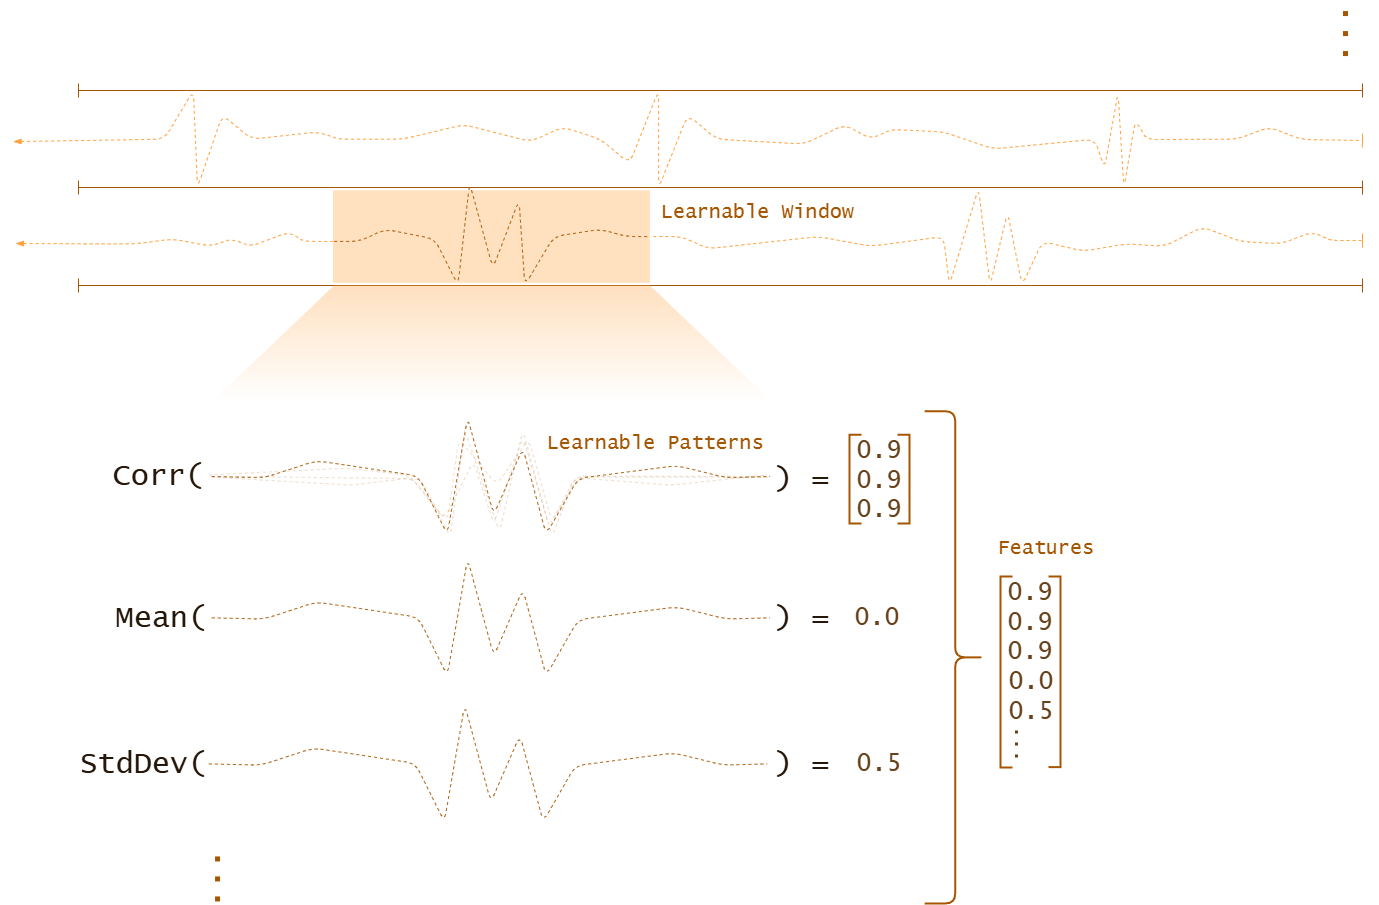
\includegraphics[width=1.0\textwidth]{sps.drawio.png}
    \caption{Spatiotemporal Sampling.}
    \label{fig:sps}
\end{figure}

The concept of spatiotemporal sampling was motivated by the physiological phenomenon known as electromechanical delay (EMD) — the latency between muscle activation and observable movement \cite{ngeo2014continuous}. In this work, we operate under the assumption that the \textit{Observed EMD} can be expressed as:
\[
\text{Observed EMD} = \text{Natural EMD} + \text{Pose Input Lag} - \text{Signal Input Lag}
\]
where each component is treated as a near-constant, assuming the variances introduced are relatively small and stable. In particular, achieving consistent input lags requires the use of precise hardware clocks, while the absence of system overloads ensures no timing drain during data acquisition. Natural EMD is considered physiologically stable and is expected to drift so slowly over time that it remains practical to compensate for it through periodic recalibration. This formulation implies a consistent and reliable temporal alignment between muscle activation and resulting motion. Therefore, if a spatiotemporal pattern is detected within a learned temporal slice, it can be reasonably assumed that a corresponding physical movement is occurring at the same moment in real life. This justifies the model's use of focused, learnable windows instead of uniformly sliding ones.

Complementing this modeling approach is the development of a new multimodal data acquisition pipeline that overcomes the cost, complexity, and fidelity barriers of existing systems. The proposed system includes:
\begin{itemize}
    \item Continuous 30fps tracking of finger joint angles using triangulated 2D projections from MediaPipe Hands across multiple synchronized RGB cameras.
    \item Real-time inverse kinematics for reconstructing full 3D hand pose from tracked keypoints.
    \item A custom-built, low-cost EMG acquisition system with six channels sampled at up to 2kHz with 12-bit resolution, supporting synchronized multimodal capture.
\end{itemize}

Together, these contributions fill a critical research gap. On the one hand, they provide a practical and scalable way to collect high-quality, long-duration sEMG and hand motion data under realistic conditions. On the other, they offer a new modeling paradigm that is capable of leveraging the rich spatiotemporal structure in such data. Notably, the new dataset is specifically designed to enable the study of intra-subject generalization over complex and continuous hand motions — an area underexplored in prior work that predominantly focuses on predefined gesture classification in short trials \cite{salter2024emg2pose}.

To demonstrate the generalizability of the proposed method, experiments were conducted both on the newly collected dataset and an existing public benchmark. These evaluations show the potential of spatiotemporal sampling to improve performance in realistic, continuous-use scenarios—advancing the state of the art in sEMG-based hand pose estimation.

\section{Purpose and Objectives}

The purpose of this thesis is to explore and validate a novel modeling and data acquisition framework for sEMG-based hand pose estimation that enables:
\begin{itemize}
    \item Learning flexible, informative spatiotemporal features from multichannel sEMG signals.
    \item Capturing hand motion data aligned with sEMG activity through a cost-efficient system.
    \item Investigating the limits of intra-user generalization over prolonged and varied motion sequences.
    \item Benchmarking the proposed model on both existing datasets and newly collected data.
\end{itemize}

To achieve this, the specific objectives include:
\begin{enumerate}
    \item Designing and implementing the Spatiotemporal Sampling model.
    \item Developing a synchronized multimodal hand tracking and EMG capture system.
    \item Conducting long-session experiments to collect a novel dataset with diverse motion patterns.
    \item Evaluating the model on both the new dataset and a public benchmark dataset.
\end{enumerate}

\section{Significance and Implications}

This thesis presents a new approach for modeling temporal and spatial characteristics of sEMG signals for hand pose estimation. The proposed method uses spatiotemporal sampling to extract a learned pattern from multichannel EMG input and measure its similarity to the signal within a learned temporal window.

In parallel, the introduced dataset capture system bridges a critical gap between cost, usability, and data fidelity. It enables researchers and developers to collect high-quality EMG and motion data without relying on prohibitively expensive commercial setups \cite{quivira2018translating}.

Testing the proposed model on both a public dataset and the custom-built multimodal dataset provides an initial evaluation of its performance and applicability under different data collection conditions. These developments contribute to the broader research efforts in wearable systems, personalized rehabilitation, and human-machine interaction.
